\documentclass[12pt,a4paper]{article}


\usepackage{macros}

\begin{document}\thispagestyle{empty}

\centerline{\Large \bf Homework 5: Due at class on April 2}



\vspace{.5cm}
\noindent  \textbf{1}. Let $ds^2=-dt^2+dx^2+dy^2$ be the Minkowski metric on $\bR^{1,2}$ and $-t^2+x^2+y^2=-1$ for $t>0$ be the space-like surface (hyperboloid $\mathbf{S}$). (See Figure 1.) Find the induced metric on the hyperboloid $\mathbf{S}$ in terms of the polar coordinate
\begin{align}
t&=r \cosh \rho  \cr
x&=r\sinh\rho\cos\phi\cr
y&=r\sinh\rho \sin\phi\nonumber
\end{align}
Given this metric, find geodesics on $\mathbf{S}$ and compute its Riemann, Ricci and scalar curvature.






\begin{figure}[h]
  \begin{minipage}[b]{8cm}\centering
 \includegraphics[width=8cm]{hyperboloid}
\caption{Hyperboloid and Poincare disk}\label{hyperboloid}
\end{minipage}
  \begin{minipage}[b]{8cm}\centering
 \includegraphics[width=6.5cm]{hyperboloid2}\label{hyperboloid2}
 \caption{Hyperboloid and Poincare disk}
\end{minipage}
\end{figure}

\begin{figure}[h]\centering
 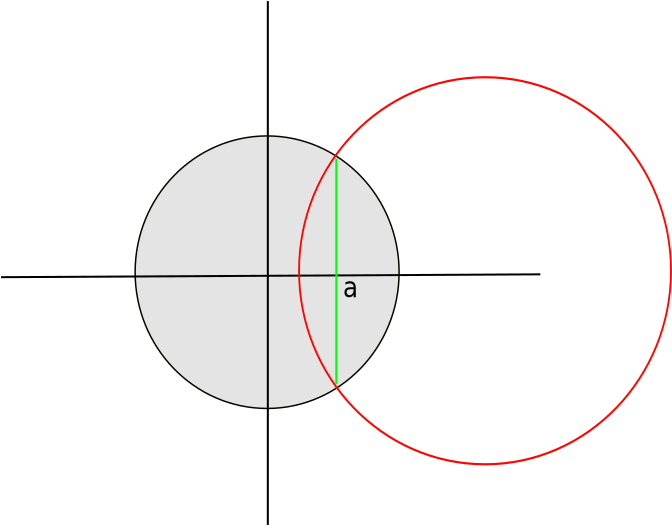
\includegraphics[width=5cm]{disk}
\caption{Poincare disk}\label{disk}
\end{figure}





\vspace{.5cm}
\noindent  \textbf{2}. Let us consider the unit disk $\mathbf{D}$ on the x-y plane. Let $\pi(P)$ be the intersection point of the unit disk and the line between the  point $(0,0,-1)$ and $P\in \mathbf{S}$. By assigning $\pi(P)$ to $P$, there is one-to-one map from the unit disk $D$ and the hyperboloid $\mathbf{S}$.
Show that the map $\pi^{-1}:\mathbf{D}\to \mathbf{S}$ is determined by
$$
(u,v) \mapsto \left(\frac{2u}{1-u^2-v^2},\frac{2v}{1-u^2-v^2},\frac{1+u^2+v^2}{1-u^2-v^2} \right)~.
$$
Find the metric on the unit disk pull-backed by this map. The unit disk $\mathbf{D}$ with this induced metric is called the Poincar\'e disk.

The red curve on the hyperboloid is an intersection with a plane (pink in Figure \ref{hyperboloid},\ref{hyperboloid2}) that goes through the origin. We put a disk (called Klein's disk) on the bottom of the hyperboloid, which allows us to get the corresponding straight line (green) on Klein's disk. This curve is mapped by $\pi:\mathbf{S}\to \mathbf{D}$ to an (red) arc in the Poincare disk. If the green line is represented by $x=a$ (Figure \ref{disk}), find the equation for the red curve.

Find geodesics on $\mathbf{D}$ and compute its Riemann, Ricci and scalar curvature.

\begin{figure}[ht]
\centering
 \includegraphics[width=6.5cm]{Poincare-upper}
 \caption{Hyperboloid and Poincare disk}\label{Poincare-upper}
\end{figure}


\begin{figure}[ht]
\centering
 \includegraphics[width=\textwidth]{triangle-upper}
 \caption{triangle in the upper half plane}\label{triangle-upper}
\end{figure}


\vspace{.5cm}
\noindent  \textbf{3}. Let $\mathbf{H}=\{(x,y)|y>0\}$ be the upper half plane (light blue area in Figure \ref{Poincare-upper}). We invert the upper half plane $\mathbf{H}$ to $\mathbf{D}$ in terms of the circle with radius $\sqrt{2}$ around the center $(0,-1)$, and take the reflection with respect to $x$-axis (Figure \ref{Poincare-upper}). This gives a map $J:\mathbf{H}\to \mathbf{D};(x,y)\mapsto(u,v)$
$$
u=\frac{2x}{x^2+(y+1)^2}~,\qquad v=1-\frac{2(y+1)}{x^2+(y+1)^2}~.
$$
\begin{enumerate}
\item Find the induced metric on the upper half plane by this map.
\item Find geodesics on $\mathbf{H}$ and compute its Riemann, Ricci and scalar curvature.
\item Find the area of the triangle with angles $(\alpha, \beta,\gamma)$ bounded by half-circles with respect to the metric (Figure \ref{triangle-upper}). Here, we can use the fact that the area of the triangle in the left of Figure \ref{triangle-upper} is the same as that of the triangle in the right of Figure \ref{triangle-upper}. Compare with the area of a triangle on the 2-sphere (Homework 1).
\item  Do parallel transport of a vector along the triangle with respect to the Levi-Civita connection of the metric and find the angle difference when it comes back. Describe the difference between the sphere and the upper half plane.
\item The \textbf{M\"obius transformation} of the upper half plane $\mathbf{H}=\{z=x+iy~|~y>0\}$  is a rational function of the form
$$f(z) = \frac{a z + b}{c z + d}~,$$
where $ad-bc=1$ with $a,b,c,d\in \bR$.  If $f_1$ and $f_2$ are M\"obius transformations, prove
that $f_1 \circ f_2$ is also a M\"obius transformation. Show that this is an isometry group for the metric.
\end{enumerate}



%\vspace{.5cm}
%\noindent  \textbf{3}. (Kepler's two-body problem)
%
%Let us consider one of the first examples of integrable systems solved by the Liouville theorem: The Kepler two-body problem of planetary motion.
%Taking the center-of-mass frame, the potential $V(r)$ of the system depends only on the radius, and the Hamiltonian is given by
%$$
%H=\frac{1}{2} \sum_{i=1}^{3} p_{i}^{2}+V(r)~.
%$$
%
%\begin{enumerate}\item Show that the angular momentum
%$$
%\vec{J}=\left(J_{1}, J_{2}, J_{3}\right), \quad J_{i j}=x_{i} p_{j}-x_{j} p_{i}=\epsilon_{i j k} J_{k}
%$$
%is conserved.
%
%\item Given the standard symplectic form $\omega=\sum_{i=1}^3dp_i\wedge dx_i$, compute the Poisson brackets
%$$
%\left\{J_{i}, J_{j}\right\}=-\epsilon_{i j k} J_{k}~.
%$$
%Show that the following three physical quantities commute under the Poisson bracket
%$$
%H, \quad J_{3}, \quad J^{2}=J_{1}^{2}+J_{2}^{2}+J_{3}^{2}
%$$
%\item  Rewrite the Liouville 1-form
%\begin{equation}\label{Liouville}
%\alpha=\sum_{i} p_{i} d x_{i}=p_{r} d r+p_{\theta} d \theta+p_{\phi} d \phi
%\end{equation}
%in terms of the polar coordinates
%$$
%x_{1}=r \sin \theta \cos \phi, \quad x_{2}=r \sin \theta \sin \phi, \quad x_{3}=r \cos \theta~.
%$$
%Rewrite the conserved quantities $H$, $J_{3}$, $J^{2}$ in terms of the polar coordinates and $(p_{r},p_{\theta},p_{\phi})$.
%
%\item Without loss of generality, we can rotate our coordinate system such that in a new system $\vec{J}$ has only the third component: $\vec{J}=\left(0,0, J_{3}\right)$. This can be simply done by setting $\theta=\frac{\pi}{2}$. Kepler's 2nd law states that the areal (sectorial) velocity is constant, and in this situation, it is nothing but the conservation of $J_3$ because the areal velocity is
%$$
%\frac{dA}{dt}=\frac12r^2\dot\phi=\frac12J_3~.
%$$
%
%
%
%Under this situation, show that an integral of the Liouville 1-form \eqref{Liouville} becomes
%\begin{equation}
%S=\int\alpha=\pm\int^{r} dr \sqrt{2(H-V)-\frac{J^{2}}{r^{2}}}+\int^{\phi} J_3 d \phi
%\end{equation}
%where the sign $\pm$ is chosen in such a way that it is consistent with $p_r$.
% Derive the equations of motion for the angle variables $$\psi_{H}=\frac{\partial S}{\partial H}, \quad \psi_{J}=\frac{\partial S}{\partial J}~.$$ Discuss their physical consequence. In particular, under which condition is an orbit of the motion closed?
%
%\item Let us assume that the potential takes the form $$V(r)=-\frac{k}{r}~.$$ Show the Kepler's 1st law: a planet describes an ellipse with the Sun at one focus.
%Let $T$ be the revolution period of a planet and $a$ be the major semi-axes of ellipse. Show the   Kepler's 3rd law:
%$$ T =\frac{2\pi}{\sqrt{k}}a^{\frac 32} ~.$$
%Refer to \href{https://en.wikipedia.org/wiki/Semi-major_and_semi-minor_axes}{Wikipedia page} for the terminolgy.

%\end{enumerate}

\end{document}
